\section{SCR-ASC System Dynamics Under Catalyst Satuaration}
The SCR-ASC subsystem in the diesel engine after-treatment systems involves reacting flow on the top of a catalyst which
adsorbs ammonia from urea decomposition. The reaction kinetics start with the decomposition of urea into ammonia
followed by its adsorption onto the surface of the catalyst. The $NO_x$ entering the chamber is reduced by this adsorbed
ammonia. The Eley-Rideal reaction mechanism \cite{yuan2015diesel}, \cite{hsieh2011development}, \cite{nova2014urea} is
considered for modeling the SCR reaction kinetics, where one reactant $(NO_x)$ is gaseous, and the other is adsorbed on
the catalyst surface $(NH_3)$. \cite{nova2014urea} lists all the reactions that take place inside the
SCR-ASC chamber. Ammonia oxidation (AMOX) happens both on the surfaces of the SCR catalyst and the ASC catalyst in the
mechanism that is similar, but SCR catalyst favors $NO_x$ reduction while ASC is specifically designed for ammonia
oxidation.
In order to keep the model order reasonably low and parameters identifiable, only the following three prominent reactions \cite{devarakonda2008adequacy},\cite{hsieh2011development} are considered:
\begin{enumerate}
    \item Standard SCR reaction:
    \begin{align*}
        4 NH_3 ^{ads} + 4 NO + O_2 &\xrightarrow[]{k_{scr}} 4 N_2 + 6 H_2O %\label{eqn::std_scr}
        & \lrf{1}
    \end{align*}
    \item Ammonia Oxidation:
    \begin{align*}
        4 NH_3^{ads} + 3 O_2 &\xrightarrow[]{k_{oxi}} 2 N_2 + 6 H_2O %\label{eqn::amox}
        & \lrf{2}
    \end{align*}
    \item Ammonia Adsorption/Desorption:
        \begin{align*}
            NH_3 + \Theta_{free} &\xrightleftharpoons[k_{des}]{k_{ads}} NH_3^{ads}
            %\label{eqn::ads}
            & \lrf{3}
        \end{align*}
\end{enumerate}

This aggregation of reactions results in errors in parameter estimates, specifically parameters containing rate constant
for the $NO_x$ reduction $\lr{k_{scr}}$ will have higher (bounded) uncertainty as it becomes dependent on the nitrogen
selectivity of AMOX reaction \cite{jain2023diagnostics}.

%=======================================================================================================================
\begin{figure}[ht]
    \centering
    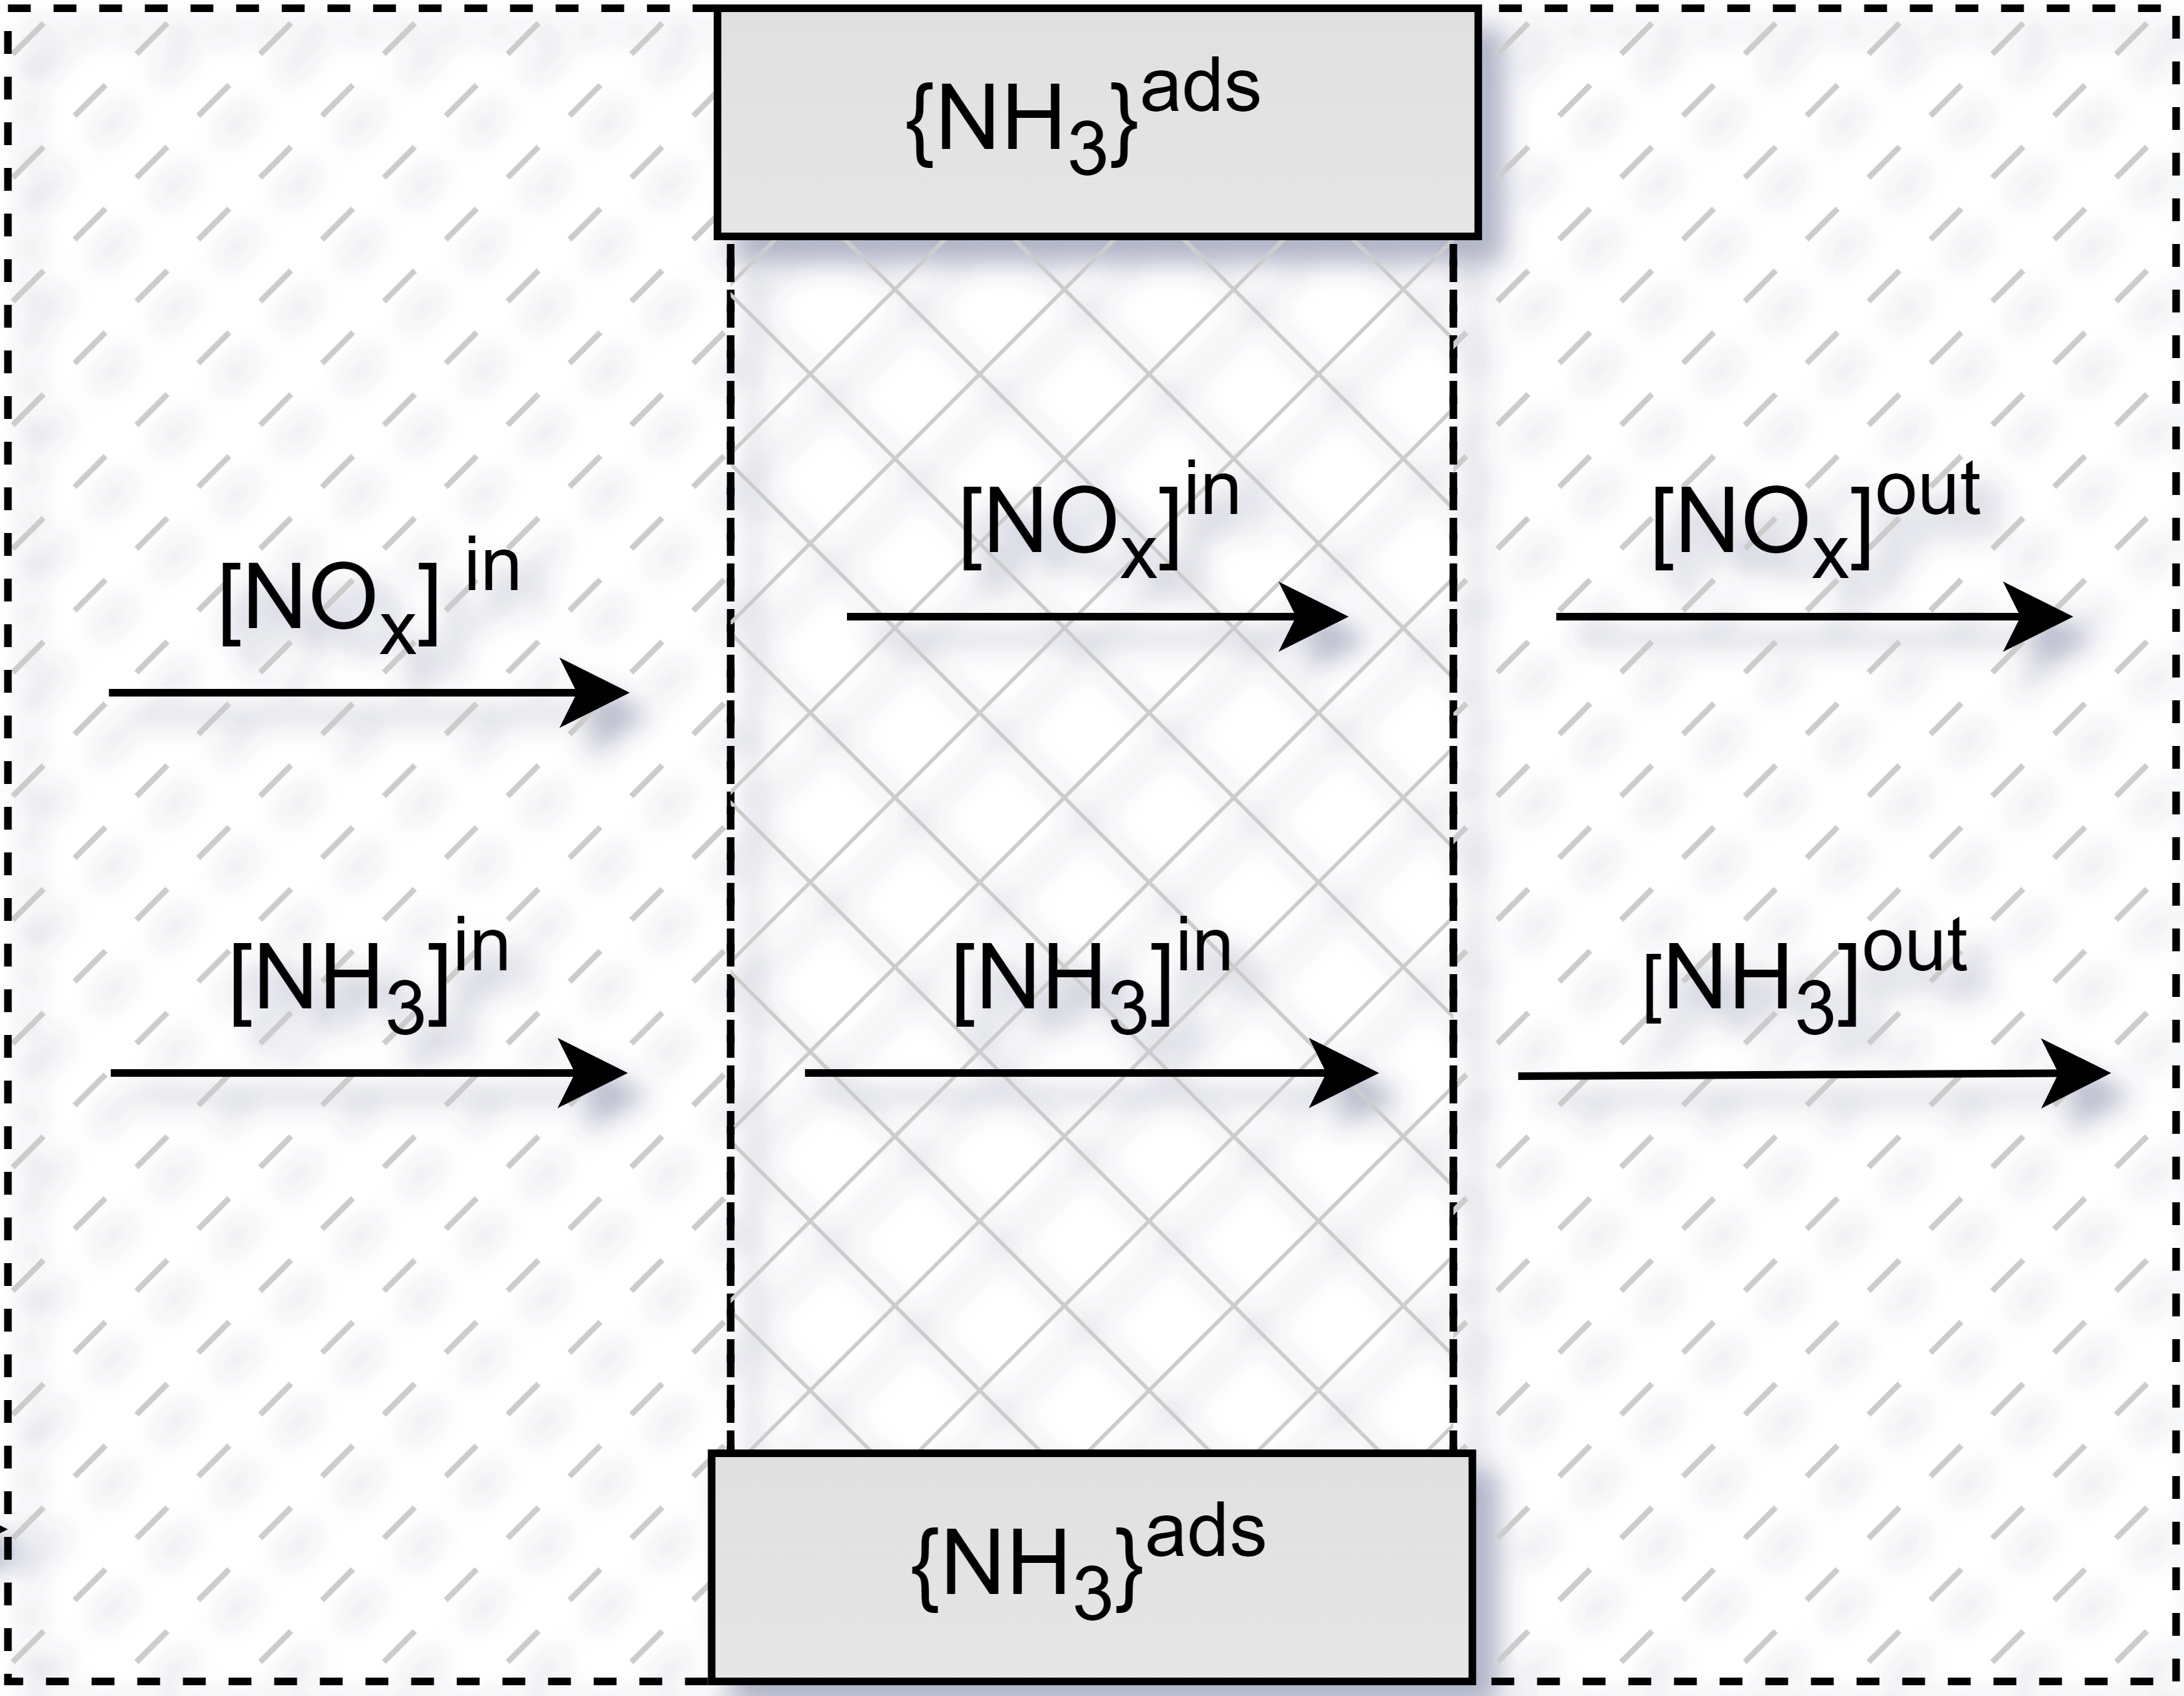
\includegraphics[width=0.35\textwidth]{figs/2_mdl/plug_flow_discrete.png}
    \caption{Approximating the plug flow reaction}
    \label{fig:plug-flow}
\end{figure}
%===
Considering the reaction chamber as a control volume (Figure-\ref{fig:plug-flow}), the dynamic model is developed based
on the molar conservation of species at the inlet and outlet separated by a residence-time interval. By assuming a
zero-order hold on the inlet species over the sampling time, the equations relating inlet and outlet concentrations at
the residence-time scale are extended to the sampling-time scale.
%====
% ======================================================================================================================
% \subsection{$NO_x$ PROCESS DYNAMICS}
Let, $\lrf{\bullet}$ be the number of moles and $\lrb{\bullet}$ be the concentration of a given species $\bullet$. We have the molar conservation of $NO_x$ across the control volume $(V_{scr})$ within one residence time $(\tau)$:
%====
\begin{multline}
        \mol{NO_x}^{out} (t + (i+1) \tau) =
                \mol{NO_x}^{in} (t + i \tau) \\
                + V_{scr} \int_0^{\tau} \frac{d}{dt} \con{NO_x}^{scr}dt
        \label{eqn::nox_bal}
\end{multline}
%===
The number of moles entering at the inlet and leaving at the outlet can be written as a function of the concentration, residence time and volume flow rate $(F_{vol})$:
%===
\begin{align}
    \mol{NO_x}^{in/out} = \con{NO_x}^{in/out} \tau F_{vol} = \con{NO_x}^{in/out} V_{scr}
\end{align}
%===
Using Eiley-Rideal mechanism for Standard SCR reaction $\lrf{2}$:
\begin{align}
    \frac{d}{dt} \con{NO_x}^{scr}dt = -k_{scr} \con{NH_3}^{ads} \con{NO_x}^{in}
\end{align}
%===
Rewriting (\ref{eqn::nox_bal}) in terms of concentrations and integrating to residence time:
\begin{multline}
        \con{NO_x}^{out} (t + (i+1) \tau) =
                \con{NO_x}^{in} (t + i \tau) \\
                -\tau k_{scr} \con{NH_3}^{ads} \con{NO_x}^{in}
        \label{eqn::nox_bal_con}
\end{multline}
%====
Summing the equations from (\ref{eqn::nox_bal_con}) for  $i = 0$ to $n-1$, where $n$ is the total number of residence times within one sampling period $(n= t_s/\tau)$ and using the zero-order hold assumptions at the inlet (\ref{eqn::zero_in}) and outlet (\ref{eqn::zero_out}) concentrations, we get equation (\ref{eqn::nox_avg}).
\begin{align}
    \con{NO_x}^{in} (t + i \tau) &= \con{NO_x}^{in}(t) \quad \forall i \in [0, n-1]  \label{eqn::zero_in}\\
    \con{NO_x}^{out} (t + (i+1) \tau) &= \con{NO_x}^{out}(t + t_s) \quad \forall i \in [0, n-1] \label{eqn::zero_out}
\end{align}
\begin{multline}
        \underbrace{\con{NO_x}^{out}}_{x_1(k+1)}(t+t_s) =
                \underbrace{\con{NO_x}^{in}}_{u_1(k)}(t) \\
                - \tau(t) k_{scr}(t) \con{NO_x}^{in}(t) \underbrace{\lrf{\frac{1}{n} \sum_{i = 0}^{n-1} \con{NH_3}^{ads}(t + i \tau)}}_{\sigma(k)}
        \label{eqn::nox_avg}
\end{multline}

% ======================================================================================================================

The quantity $\sigma(k)$ is the average concentration of ammonia adsorbed on the catalysts surface across the $n$ residence times between $k$ and $k+1$ samples. $\sigma(k)$ is bounded by the total concentration of voids on the surface of the catalyst, $\Gamma$, which decrease with increase in temperature.
\begin{align}
    0 \leq \sigma(k) \leq \Gamma \qquad \forall k
\end{align}
%===
The unbounded dynamics of $\sigma$, $\sigma^{ub}(k)$ is a nonlinear function dependent on concentration of adsorbed ammonia, urea dosing $\lr{u_{inj}}$, and the inlet $NO_x$ concentration from the previous time step.
\begin{align}
    \sigma^{ub}(k) &= g_{\sigma} \lr{ \sigma(k-1), u_{inj}(k-1), \con{NO_x}^{in}(k-1) }
\end{align}
The actual expression, which is beyond the scope of this work, can be derived using the similar approach used for
deriving $NO_x$ process dynamics (\ref{eqn::nox_avg}). $\sigma(k)$ can be described using the following pairwise
function:
\begin{align}
    \sigma(k) &=
    \begin{cases}
        \sigma^{ub}(k) & \text{if } \quad 0 \leq \sigma^{ub}(k) \leq \Gamma \\
        \Gamma         & \text{if } \quad \sigma^{ub}(k) > \Gamma \qquad \text{[Satuaration]}\\
        0              & \text{if } \quad \sigma^{ub}(k) < 0 \qquad \text{[Empty]}
    \end{cases}
\end{align}
%===
Thus, for $NO_x$ process dynamics under catalyst saturation, $\sigma(k) = \Gamma$. From (\ref{eqn::nox_avg})
\begin{align}
    x_{1_{sat}}(k+1) &= u_1(k) - \tau(k) k_{scr}(k) u_1(k) \Gamma
        \label{eqn::nox_mdl}
\end{align}
%===
Defining $\eta(k)$ as change in $NO_x$ concentration reduction during the time between $k-1$ and $k$, i.e.,
\begin{align}
    \eta_{sat}(k) &= u_1(k-1) - x_{1_{sat}} (k)
    \label{eqn::eta}
\end{align}
%===
The residence time can be parameterized as a function of mass flow rate $\lr{F}$ assuming that the effect of the density variation on residence time is insignificant.
\begin{align}
    \tau(k) &= \frac{\rho V_{scr}}{F} = \frac{\tau_0}{F}
    \label{eqn::res_time}
\end{align}
%===
The temperature dependence of the rate constant, $k_{scr}$, can be approximated by linearizing Arrhenius equation as:
\begin{align}
    k_{scr}(T) = A_{scr} e^{\lr{-\frac{E_{scr}}{RT}}} \approx k_1 T + k_0 \qquad k_1, k_0 > 0
    \label{eqn::rate_const}
\end{align}
%===
The temperature model for concentration of viable voids $\Gamma$ on the catalyst is approximated as a linear function that decreases with increase in temperature.
\begin{align}
    \Gamma(T) &\approx -\gamma_1 T + \gamma_0 \qquad \gamma_1, \gamma_0 > 0
    \label{eqn::gamma}
\end{align}
%===
Incorporating equations (\ref{eqn::eta}), (\ref{eqn::res_time}) and (\ref{eqn::gamma}) into the $NO_x$ process dynamic model (\ref{eqn::nox_mdl}) and writing in regression form, we get
\begin{align}
    \eta_{sat}(k+1) &= \pmb \phi_{sat}^T(k) \pmb \theta_{sat}
    \label{eqn::regression} \\
    %===
    \pmb \phi_{sat} (k) &= \frac{u_1(k)}{F(k)} \times \bm{T^2 \\ T \\ 1}
    \label{eqn::phi_def}\\
    %===
    \pmb \theta_{sat} &= \tau_0 \times \bm{-k_1 \gamma_1 \\ k_1 \gamma_0 - k_0 \gamma_1 \\ k_0 \gamma_0}
                       = \bm{\theta_1 \\ \theta_2 \\ \theta_2}
    \label{eqn::theta_def}
\end{align}

%===
Based on the parameter definitions (\ref{eqn::theta_def}), the signs of two of the parameters is deterministic.
\begin{align}
    \theta_1 \leq 0, \qquad
    \theta_3 \geq 0
\end{align}
